\documentclass[12pt]{article}

\usepackage[T1]{fontenc}
\usepackage[french]{babel}
\usepackage[utf8]{inputenc}
\usepackage{lmodern}
\usepackage{pict2e}
\usepackage{graphicx}
\usepackage{float}
\usepackage{siunitx}

\title{Rapport de TP réseaux : le bus CAN}
\author{Stanislas BERNARD et Alexandre MARCIREAU}
\date{12 Janvier 2015} 

\begin{document}

\setlength{\unitlength}{1cm}

\maketitle

\section{Présentation de la maquette}

\subsection{Qu'est-ce qu'un tranceiver CAN ? A quoi sert-il ?}

Un tranceiver CAN est un composant qui se branche sur le bus CAN, et qui permet de récupérer sur une entrée/sortie série les trames circulant sur le bus. Il permet également de faire passer des trames sur le bus.

\subsection{Où est le contrôleur CAN qui crée et vérifie les CRC, compte les erreurs, construit la trame ?}

Ce contrôleur qui gère l'ensemble du protocole CAN se situe directement dans le microcontrôleur PIC18F2680.

\subsection{Qu'est-ce que la CPU doit envoyer au contrôleur CAN pour qu'il puisse émettre un message ?}

Pour émettre un message, la CPU doit envoyer l'identifiant du message, ainsi que le contenu. Le contrôleur gérera ensuite tout le reste à partir de ces données.

\subsection{Faites un schéma incluant le tranceiver CAN, la CPU, le contrôleur CAN et indiquant les échanges ente ces éléments}

\begin{figure}[H]
\centering
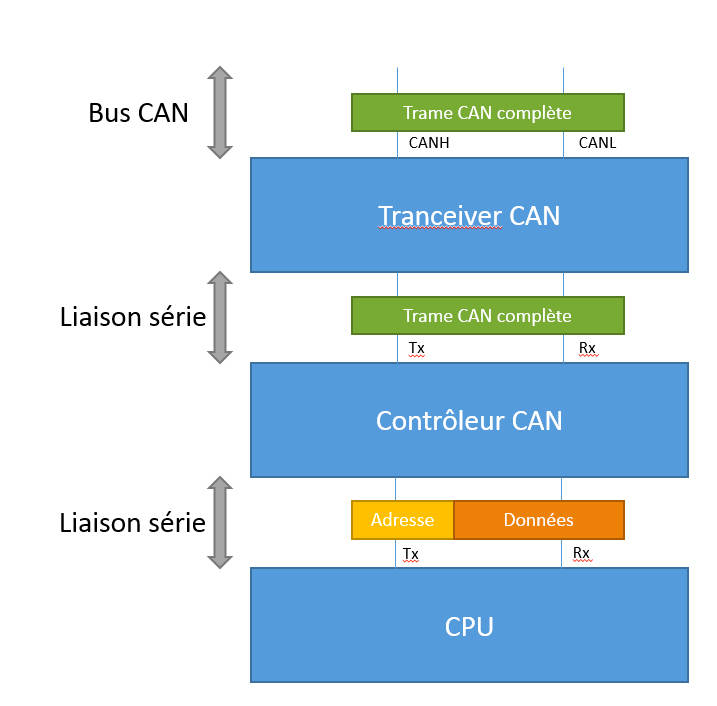
\includegraphics[width=0.7\textwidth]{schema.jpg}
\caption{Fonctionnement CPU <-> CAN}
\end{figure}

\subsection{Les trames ne transportent qu'un octet de données. Quelle est la durée approximative d'une trame ?}

Le débit de ce CAN est de $1Mbps$. Dans une trame CAN, on a $1+11+1+6+15+1+1+1+7+3+8*n_{octets}$ bits, soit ici 55 bits. La durée approximative d'une trame est donc de \SI{55}{\micro\second}.

\end{document}